% ============================================================
% CHAPTER 4: METHODOLOGY
% ============================================================
\chapter{Methodology}
\label{ch:methodology}

This chapter presents the analytical framework for classifying and evaluating the West Midlands cycling network by Level of Traffic Stress (Figure~\ref{fig:methods}). Sections~\ref{sec:method-extraction}--\ref{sec:method-junctionlts} construct the directed, stress-classified network: extracting cyclable segments from OS NGD, assigning link-level LTS, and propagating junction stress with LTN 1/20's criteria. Section~\ref{sec:method-analysis} uses this network to test connectivity against LTN 1/20's “Cycling for all” principle through density, fragmentation, and reach analyses. Section~\ref{sec:method-growth} compares three network growth strategies to inform upgrade prioritisation.

\begin{figure}[htbp]
  \centering
  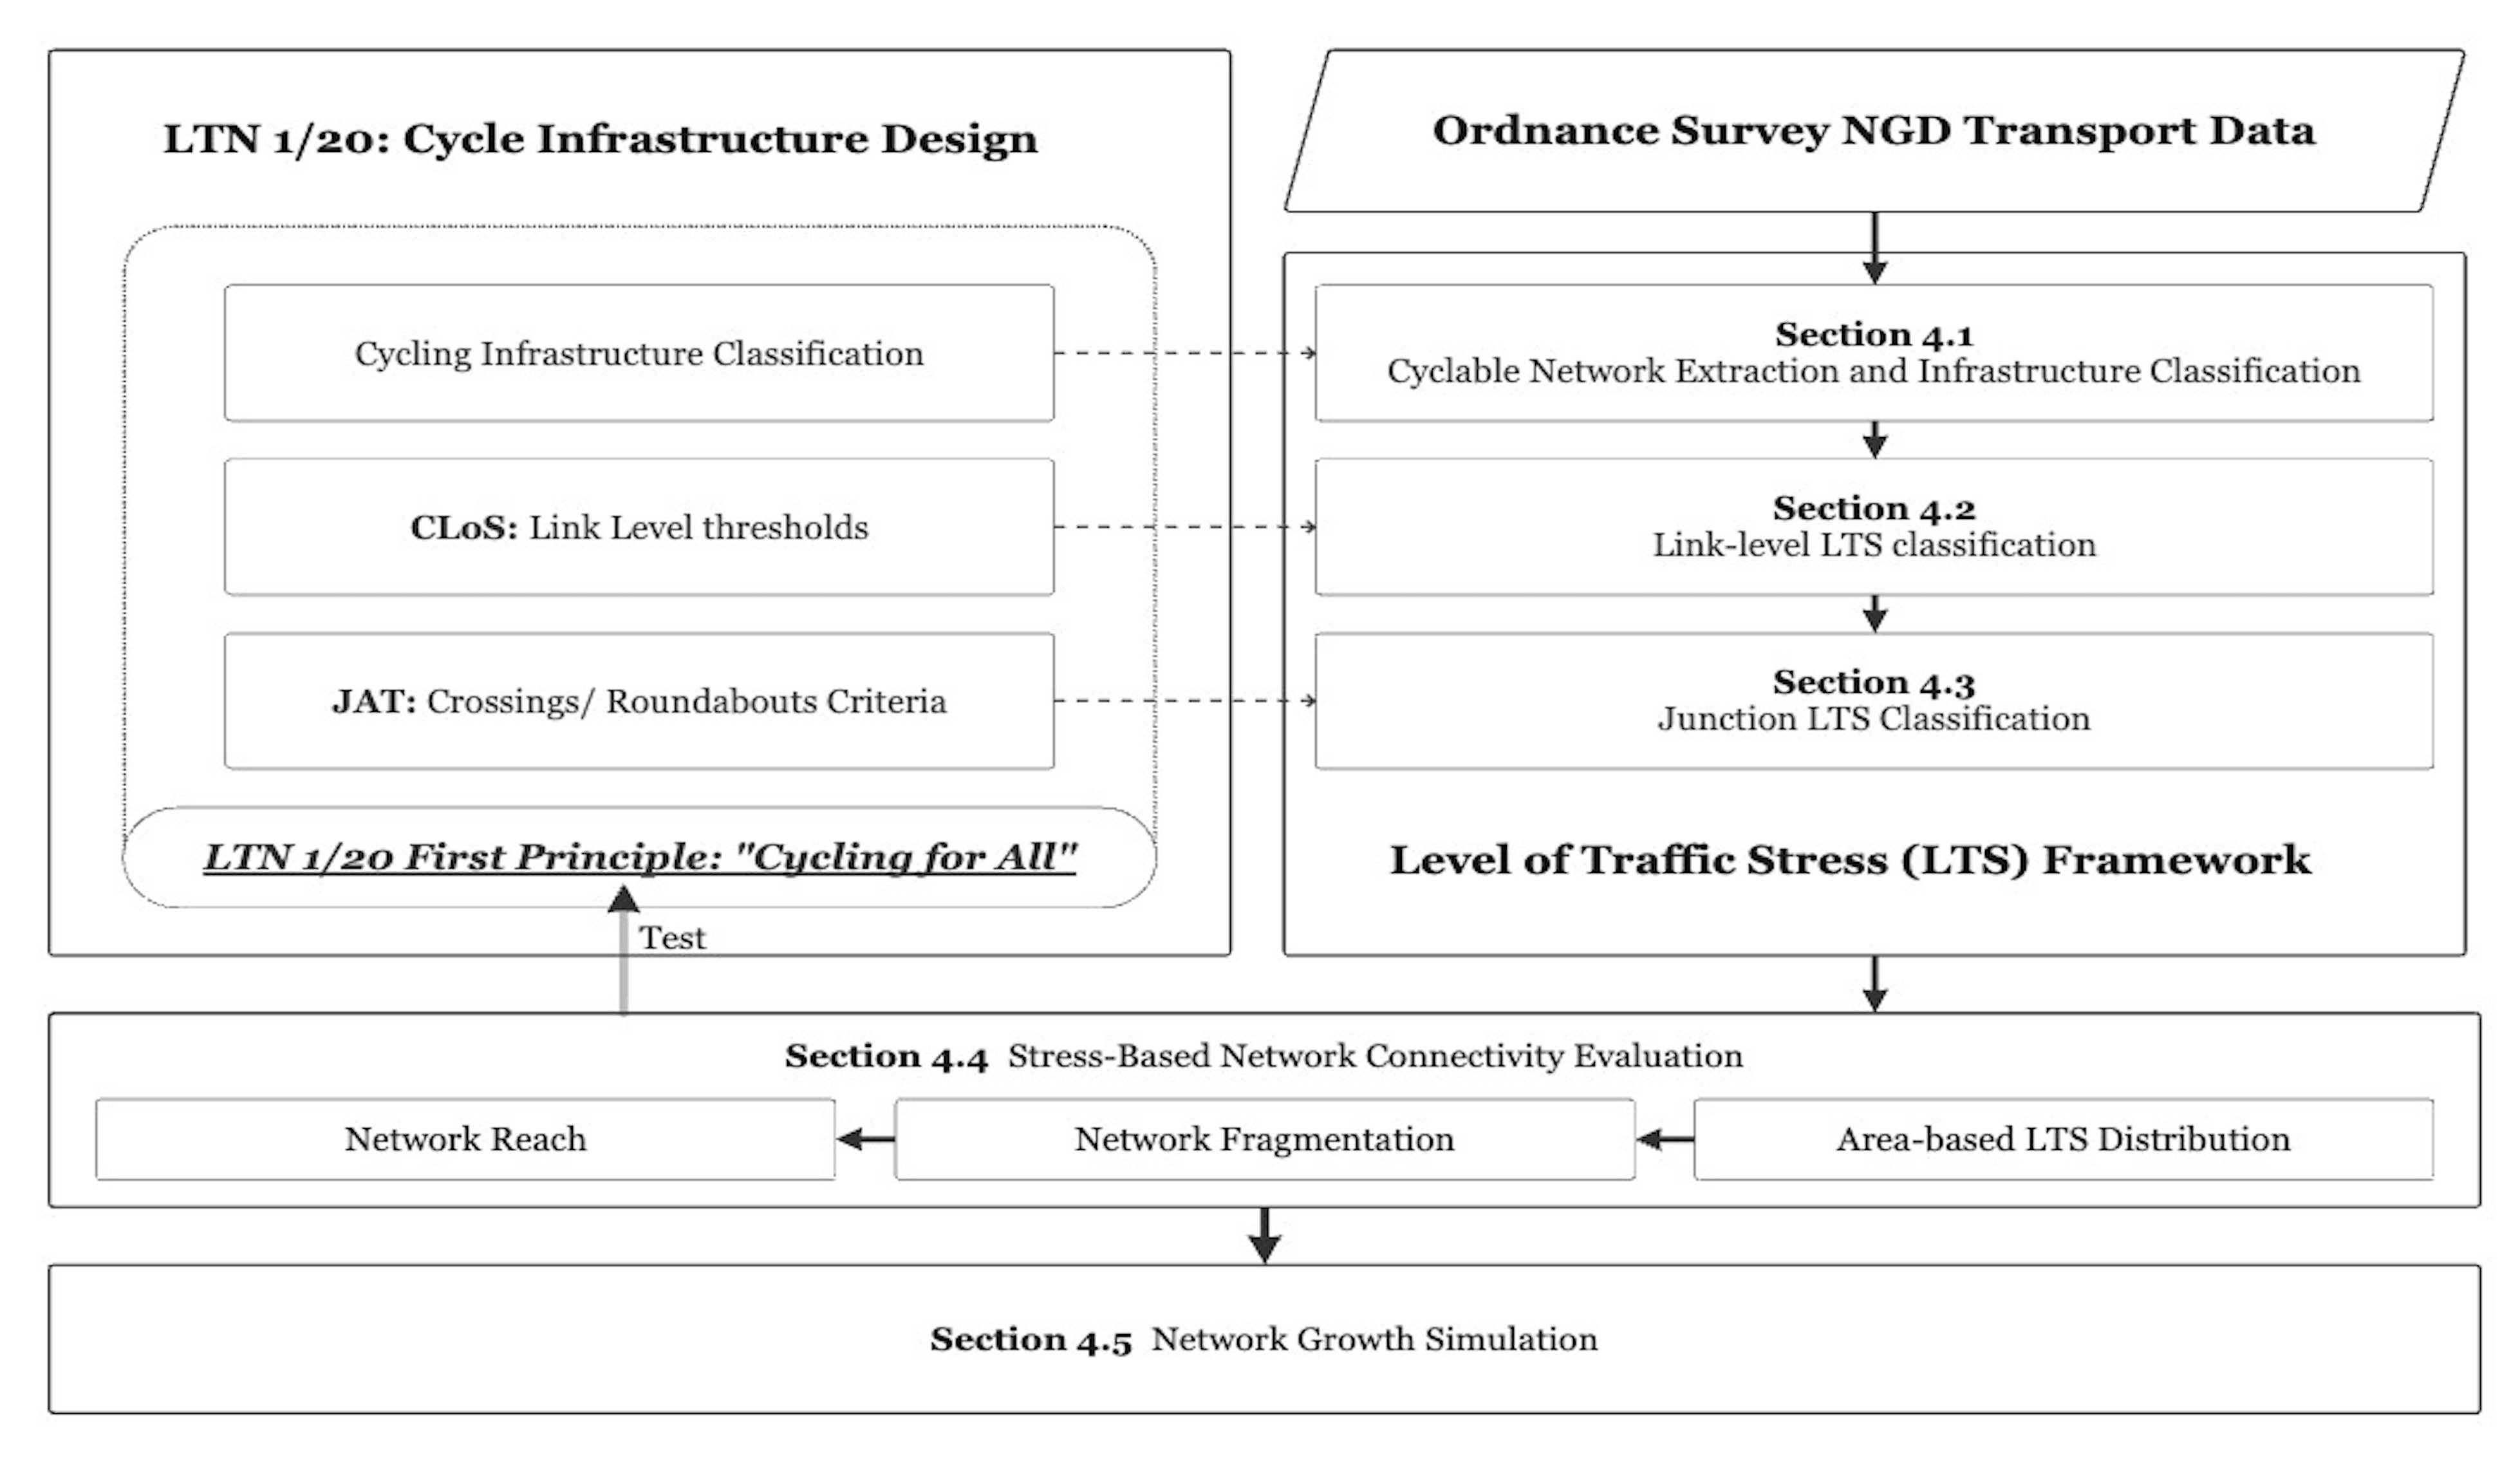
\includegraphics[width=\textwidth]{Figure/methods.jpg}
  \caption{Analytical framework. LTN 1/20 design criteria (left) supply the classification thresholds operationalised on OS NGD Transport data (right). The classified network is then evaluated against LTN 1/20's "Cycling for All" principle through connectivity analysis and network growth simulation.}
  \label{fig:methods}
\end{figure}

\section{Cyclable Network Extraction and Infrastructure Classification}
\label{sec:method-extraction}

The first stage of the classification process extracts all legally and practically cyclable segments from the West Midlands transport network. Cyclable infrastructure is represented in two feature collections under OS NGD Transport Theme: Road Links, which represent the carriageway network \parencite{ordnancesurvey2026a}, and Path Links, which represent routes topologically independent from it \parencite{ordnancesurvey2026b}. The legal cyclability of segments is firstly checked through the Highway Dedication feature collection, which provides an indication of the type of highway user who has access to each section of the network, recording one of eight designation types \parencite{ordnancesurvey2026}. Five of the seven designation types permit cycling under UK highway law, while `Motorway' and `Pedestrian Way Or Footpath' are excluded as non-cyclable (Table~\ref{tab:highway-dedication}).
 
\begin{table}[htbp]
  \centering
  \caption{Highway Dedication types and legal cyclability under UK highway law.}
  \label{tab:highway-dedication}
  \small
  \begin{tabularx}{\textwidth}{l l X}
    \toprule
    Highway Dedication & Cyclable? & Legal Basis \\
    \midrule
    All Vehicles & Yes & Cycling permitted on public roads by default \\
    Cycle Track or Cycle Way & Yes & Cycle Tracks Act 1984 \\
    Bridleway & Yes & Countryside Act 1968, s.30 \\
    Restricted Byway & Yes & Countryside and Rights of Way Act 2000 \\
    Byway Open to All Traffic & Yes & Wildlife and Countryside Act 1981, s.66(1) \\
    Motorway & No & Motorways Traffic (England and Wales) Regulations 1982 \\
    Pedestrian Way or Footpath & No & No public right of way for cycling (cf.\ Highways Act 1835, s.72) \\
    \bottomrule
  \end{tabularx}
  \par\smallskip
  \footnotesize\textit{Note:} The eighth type, `No Dedication Or Dedication Unknown', is neither cyclable nor explicitly non-cyclable and is addressed through the description-based fallback classification for Road Links.
\end{table}
 
For Road Links, Highway Dedication covers most of the segments. Where a dedication record is absent or recorded as `No Dedication Or Dedication Unknown', a fallback classification retains segments whose physical description feature indicates a carriageway type \footnote{`Single Carriageway', `Dual Carriageway', `Roundabout', `Slip Road', `Shared Use Carriageway', `Traffic Island Link At Junction', and `Traffic Island Link'.}. Segments classified as `Motorway' are excluded regardless of dedication status. This process yields 212,551 cyclable Road Links (97.8\%), of which 84.2\% are identified through Highway Dedication and 15.8\% through the description fallback. For Path Links, Highway Dedication coverage is substantially lower, identifying only 10.1\% of cyclable paths. A second layer retains paths where the feature data detects cycling infrastructure through its `presenceofcyclelane' attribute, contributing a further 1.0\%. No attribute in the OS NGD Path Link schema, however, provides a direct cyclability indicator. This mirrors DfT’s own transport connectivity metric, which uses Ordnance Survey data for the driving network but relies on OpenStreetMap tags for cycling and walking network definition \parencite{dft2025}. Following this, a third layer performs spatial cross-validation against the OpenStreetMap cycling network, matching remaining paths without Highway Dedication or cycle lane presence to OSM cycling geometries within a 5-metre nearest-neighbour spatial join and recovering an additional 40,035 paths. Paths with explicitly non-cyclable Highway Dedications are excluded at all layers. This process yields 45,023 cyclable Path Links (40.3\% of the total collection). Each segment is then expanded into directed edges, and cycle lane records are joined only to the edge whose travel direction aligns with the lane's placement side, capturing the inherently asymmetric distribution of cycling infrastructure and avoiding overestimation of facility provision.
 
Each directed cyclable segment is then classified into one of eight facility types derived from LTN~1/20's design hierarchy (Table~\ref{tab:facility-types}). The OS NGD Cycle Lane dataset, whose type definitions are aligned to LTN~1/20, records dedicated cycling infrastructure as separate features referencing their parent Road Link \parencite{ordnancesurvey2026c,ordnancesurvey2026d}. A Road Link with a matching Cycle Lane record is classified according to its cycle lane description; where multiple records exist for the same link, the more protective facility governs. Road Links without a matching record, or where the cycle lane type is recorded as `Unknown Type Of Cycle Track Or Lane', default to Mixed Traffic. All cyclable Path Links are classified as `Off-Road', as they are topologically independent from the road network and carry no motor traffic speed or volume attributes \parencite{ordnancesurvey2026b}. Following classification, Road Links and Path Links are merged into a single unified and directed network for use in the subsequent LTS assessment.
 
\begin{table}[h]
  \centering
  \caption{Facility type classification derived from LTN~1/20 design hierarchy, mapped to OS NGD data sources.}
  \label{tab:facility-types}
  \begin{tabular}{lll}
    \toprule
    Facility Type & OS NGD Source & Classification Feature \\
    \midrule
    Off-Road & Path Link & Cyclable Path Links \\
    Shared Use & Cycle Lane & `Unsegregated Shared Use Cycle Facility' / \\
     & & `Segregated Shared Use Cycle Track' \\
    Fully Kerbed Cycle Track & Cycle Lane & `Fully Segregated Cycle Track' \\
    Stepped Cycle Track & Cycle Lane & `Stepped Cycle Track Along Road' \\
    Light Segregation & Cycle Lane & `Lightly Segregated Cycle Lane On Road' \\
    Mandatory Cycle Lane & Cycle Lane & `Mandatory Cycle Lane On Road' \\
    Advisory Cycle Lane & Cycle Lane & `Advisory Cycle Lane On Road' \\
    Mixed Traffic & Road Link (main) & `Unknown Type Of Cycle Track Or Lane' or \\
     & & no matching Cycle Lane record \\
    \bottomrule
  \end{tabular}
  \par\smallskip
  \footnotesize\textit{Note:} Some facility types overlap conceptually. Off-Road paths may in practice function as shared-use routes or as kerbed cycle tracks. This does not affect the subsequent LTS classification, as all such facilities are fully separated from motor traffic.
\end{table}


\section{Link-level LTS classification}
\label{sec:method-linklts}

The link-level LTS classification adapts the \textcite{mekuria2012a} framework by replacing its North American thresholds with those from LTN~1/20. Although the CLoS tool uses compensatory scoring across heterogeneous subcriteria, which prevents it from isolating population-level acceptability (see Section~\ref{sec:lit-ltn}), the core Safety subcriteria addressing motor traffic speed (Criterion 10), volume (Criterion 11), segregation provision and carriageway width (Criterion 12) are themselves non-compensatory stress determinants constructed on CROW-derived logic \parencite{crow2016}, directly consistent with the LTS framework. This study maps that graduated logic onto the four LTS levels: conditions suitable for all users including children (LTS 1), most adults (LTS 2), confident cyclists (LTS 3), and conditions triggering a critical safety failure under LTN 1/20 criteria (LTS 4), as detailed in Table~\ref{tab:lts_matrix}.

\renewcommand{\arraystretch}{1.4}
\begin{table}[h]
\centering
\caption{Link-level LTS classification matrix derived from LTN~1/20 Safety subcriteria.}
\label{tab:lts_matrix}
\footnotesize
\begin{tabularx}{\textwidth}{
  >{\raggedright\arraybackslash}p{2.8cm}
  >{\raggedright\arraybackslash}X
  >{\raggedright\arraybackslash}X
  >{\raggedright\arraybackslash}X
  >{\raggedright\arraybackslash}X
}
\toprule
\textbf{Facility type} & \textbf{LTS~1} & \textbf{LTS~2} & \textbf{LTS~3} & \textbf{LTS~4} \\
\midrule
Off-Road              & All conditions & ---  & ---  & ---  \\
Shared Use            & All conditions & ---  & ---  & ---  \\
Fully Kerbed Cycle Track & All conditions & --- & --- & ---  \\[3pt]
Stepped cycle track   & $V_{85} \leq 30$\,mph & $V_{85}$ 30--37\,mph & $\geq 37$\,mph & --- \\
Light segregation     & $V_{85} \leq 30$\,mph & $V_{85}$ 30--37\,mph & $\geq 37$\,mph & --- \\[3pt]
Mandatory cycle lane  &
  Width $\geq 1.8$\,m,\newline $V_{85} \leq 20$\,mph,\newline AADT $\leq 5{,}000$ &
  Width $\geq 1.8$\,m,\newline $V_{85}$ 20--30\,mph,\newline AADT $\leq 5{,}000$ &
  Width $< 1.8$\,m; or\newline $V_{85}$ 30--37\,mph; or\newline AADT 5,000--10,000 &
  $V_{85} \geq 37$\,mph; or\newline AADT $\geq 10{,}000$ \\[3pt]
Advisory cycle lane   &
  Width $\geq 1.8$\,m,\newline $V_{85} \leq 20$\,mph,\newline AADT $\leq 5{,}000$ &
  Width $\geq 1.8$\,m,\newline $V_{85}$ 20--30\,mph,\newline AADT $\leq 5{,}000$ &
  Width $< 1.8$\,m; or\newline $V_{85}$ 30--37\,mph; or\newline AADT 5,000--10,000 &
  $V_{85} \geq 37$\,mph; or\newline AADT $\geq 10{,}000$ \\[3pt]
Mixed traffic         &
  $V_{85} \leq 20$\,mph,\newline AADT $\leq 2{,}500$ &
  $V_{85}$ 20--30\,mph,\newline AADT 2,500--5,000 &
  $V_{85}$ 30--37\,mph; or\newline AADT 5,000--10,000 &
  $V_{85} \geq 37$\,mph; or\newline AADT $\geq 10{,}000$; or\newline nearside lane 3.2--3.9\,m\newline and AADT $\geq 5{,}000$ \\
\bottomrule
\end{tabularx}

\vspace{0.5em}
\footnotesize
\noindent\textit{Notes:}
\begin{enumerate}[nosep, leftmargin=*, label=\arabic*.]
    \item Where multiple criteria apply to a single segment, the overall LTS is determined by the worst-performing criterion (non-compensatory).
    \item Thresholds are derived from the CLoS Safety subcriteria (Criteria 9--12, 15) in LTN~1/20 Appendix~A, supplemented by the speed--volume--facility matrix in Figure~4.1, which the CLoS itself references as complementary guidance for determining appropriate separation levels.
    \item Motor traffic volume is expressed as Annual Average Daily Traffic (AADT), used as a proxy for the passenger car unit (PCU) thresholds specified in LTN~1/20 Criterion~11. LTN~1/20 additionally specifies HGV composition thresholds ($>5\%$ for critical fail, 2--5\% for score~0); these could not be applied due to the absence of network-wide vehicle composition data and are acknowledged as a limitation (see section~\ref{sec:disc-limitations}).
    \item Rural exception: mixed traffic segments with $V_{85} \leq 30$\,mph and AADT $\leq 1{,}000$ are classified as LTS~1, following LTN~1/20 Figure~4.1 Note~3.
\end{enumerate}
\end{table}
\renewcommand{\arraystretch}{1.0}

The link-level LTS classification begins with facility type and proceeds through three primary variables: prevailing speed, road width, and motor traffic volume. OS~NGD provides carriageway or cycle lane width at the link level through average and minimum width attributes. For cycle lanes, this study uses the separately recorded modal lane width rather than the minimum, as it better captures typical conditions along a segment. For mixed traffic on single carriageways, average road width is used to assess the critical nearside lane width range of 3.2 to 3.9\,m associated with elevated close-pass risk\footnote{On one-way roads, total width serves directly as lane width; on two-way roads, lane width is approximated as half the total width, with the override applied only where AADT exceeds 5,000, as lower volumes allow drivers to overtake via the opposing lane.}. Segments triggering this override are classified as LTS~4.

Prevailing speed is represented by the estimated 85th percentile speed ($V_{85}$), consistent with the measurement basis specified in LTN~1/20. $V_{85}$ is preferred over posted speed limits as actual operating speeds frequently diverge from the limit depending on road geometry and enforcement, offering a more reliable measure of cycling stress \parencite{fitzpatrick2003, europeancommission2021, departmentfortransport2025b}. $V_{85}$ was estimated from the OS~NGD average speed dataset (RAMI), which provides mean vehicle speeds derived from probe vehicle data across multiple time periods. The mean of observed average speeds across all available time periods was used as the representative link speed, and $V_{85}$ was calculated by applying a 7/6 multiplier derived from CA~185 \textit{Vehicle speed measurement} \parencite{nationalhighways2019}, which defines $V_{85}$ as the mean speed plus one standard deviation and estimates the standard deviation as approximately one-sixth of the mean under the assumption of a normal speed distribution.

OS~NGD does not include motor traffic volume attributes. To address this, major road volumes were obtained directly from DfT annual average daily traffic (AADT) count point data, while minor road volumes were estimated following the methodology of \parencite{morley2016}. A Poisson GLM was constructed using road network characteristics extracted via pgRouting on the England OSM network as predictors and DfT count point observations as the dependent variable. Five-fold cross-validation ($n = 3{,}695$ count points) yields an $R^2$ of $0.604 \pm 0.019$ and Spearman's $\rho$ of $0.803 \pm 0.015$, considered sufficient for the coarse-grained LTS classification task. Predicted and observed AADT values were assigned to OS~NGD links via nearest-network spatial join. For the small number of links where no match was achieved, volume was imputed using the median AADT of the corresponding road classification to ensure network-wide coverage.

\section{Junction LTS Classification}
\label{sec:method-junctionlts}

The original LTS framework established intersection-specific criteria covering weaving conflicts and crossing stress, with junction stress propagated to approaching minor-street links \parencite{mekuria2012a,furth2016}. However, the fine-grained geometric data these require are unavailable at network scale \parencite{bearn2018,furth2018}, driving adoption of the \textcite{conveyal2015} method, which propagates the highest segment LTS at each unsignalized vertex to all incident edges without independently evaluating crossing geometry. This max-propagation logic has been widely applied \parencite{semler2017,murphy2019,huertas2020}, with variants introducing signal or stop sign presence as downgrading modifiers \parencite{bearn2018,lin2021}; a substantial number of studies omit junction treatment entirely \parencite{wang2022,viero2025}. Two gaps persist. First, all existing criteria address North American junction typologies and none cover roundabouts, despite their prevalence in UK networks and documented cyclist collision risk \parencite{daniels2009,aldred2021,poudel2021,rodrigues2022}. Second, undirected vertex-level propagation assigns elevated stress indiscriminately to all incident edges regardless of legal travel direction, obscuring heterogeneity in crossing conditions.

The Junction Assessment Tool (JAT) within LTN 1/20 evaluates junction suitability by
establishing criteria for each junction form (priority T-junction, crossroads,
traffic signals, roundabout), disaggregated by the specific cycle movement being
assessed. From this structure, three variables can be identified as governing
crossing stress: the speed and volume of conflicting motor traffic, which determine
the severity of the potential conflict; the number of lanes to be crossed in one movement,
which determines the duration of exposure; and the availability of protection such
as a central refuge, traffic signals, or dedicated cycle priority. LTN 1/20 also
provides a crossing design suitability matrix that classifies crossings by these
variables into three suitability tiers: suitable for most people, not suitable for
all, and suitable for few. For non-roundabout crossing junctions
(Table~\ref{tab:crossing-lts}), the present study maps these three suitability tiers
to LTS 1, LTS 2, and LTS 3--4 respectively. Protection is operationalised in three
levels: uncontrolled, traffic island (identified from the OS NGD link description
field ``Traffic Island Link At Junction\footnote{The OS NGD does
not distinguish between median refuges, central islands, and other refuge forms, but
the presence of a traffic island at a junction at minimum serves to channelise
traffic flow and provide physical separation.}''), and signalized (identified from
OpenStreetMap traffic signal tags spatially joined to OS NGD nodes).  For roundabouts
(Table~\ref{tab:roundabout-lts}), the classification is derived directly from the JAT
roundabout-specific criteria, which assess suitability by traffic throughput,
approach geometry, and off-carriageway cycle facility provision. Each roundabout is classified by the maximum AADT, V85, and road width of its incident links.

\begin{table}[htbp]
  \centering
  \caption{Crossing Junction LTS Classification}
  \label{tab:crossing-lts}
  \begin{tabularx}{\textwidth}{X X X c c c}
    \toprule
    & & & \multicolumn{3}{c}{LTS by protection level} \\
    \cmidrule(lr){4-6}
    V85 (mph) & AADT & Est.\ lanes & Uncontrolled & Traffic island & Signalised \\
    \midrule
    $\geq$ 37   & Any            & Any      & 4 & 4 & 3 \\
    30--37      & $>$ 10,000     & Any      & 4 & 4 & 1 \\
    30--37      & 6,000--10,000  & $\geq$ 2 & 4 & 4 & 1 \\
    30--37      & $\leq$ 6,000   & $\geq$ 2 & 3 & 3 & 1 \\
    30--37      & $\leq$ 10,000  & 1        & 2 & 2 & 1 \\
    $\leq$ 30   & $>$ 8,000      & $>$ 2    & 4 & 3 & 1 \\
    $\leq$ 30   & $>$ 8,000      & $\leq$ 2 & 3 & 2 & 1 \\
    $\leq$ 30   & 4,000--8,000   & $\geq$ 2 & 2 & 2 & 1 \\
    $\leq$ 30   & 4,000--8,000   & 1        & 2 & 1 & 1 \\
    $\leq$ 30   & $\leq$ 4,000   & $\geq$ 2 & 2 & 1 & 1 \\
    $\leq$ 30   & $\leq$ 4,000   & 1        & 1 & 1 & 1 \\
    \bottomrule
  \end{tabularx}
\end{table}

\begin{table}[htbp]
  \centering
  \caption{Roundabout LTS Classification}
  \label{tab:roundabout-lts}
  \begin{tabularx}{\textwidth}{X c}
    \toprule
    Base conditions & LTS \\
    \midrule
    AADT $>$ 8,000 AND est.\ lanes $\geq$ 2; OR V85 $\geq$ 37 mph & 4 \\
    AADT $>$ 8,000 OR est.\ lanes $\geq$ 2 (but not both)         & 3 \\
    All other roundabouts (compact/mini, AADT $\leq$ 8,000)       & 2 \\
    Segregated cycle facility AND traffic signal                  & 1 \\
    \bottomrule
  \end{tabularx}

  \smallskip
  {\footnotesize \textit{Note.} When traffic lights are present, the LTS value is
  reduced by one level to a minimum of LTS 2.}
\end{table}

The junction classification operates at the (link, junction node) pair level. The
JAT defines junction stress in terms of cycle movements ``in potential conflict''
with motor traffic, where conflict arises from traffic streams that cross or run
alongside the cyclist's path without being separated physically or in time.
Following this definition, the present study identifies conflicting links at each
crossing junction via the OS NGD directionality attribute, retaining only those that
a cyclist departing the node could legally enter, and further excluding straight-line
continuations of the approach link through a bearing-based filter (departure bearing
within $180^{\circ} \pm 30^{\circ}$, a threshold following the orientation criterion in
\textcite{mekuria2012a}). The three crossing variables (maximum V85, maximum AADT,
and maximum estimated lane count) are then taken from the remaining conflict links,
ensuring all three reflect the transverse traffic stream being crossed. For
roundabout nodes, where circulatory geometry renders approach-level analysis
inapplicable, the classification operates at the node level using the maximum
traffic attributes across all incident links. In both cases, the junction LTS is
overlaid onto the segment classification using worst-indicator-wins logic, so that
junction stress can only elevate the final LTS of a link.

\section{Stress-Based Network Connectivity Evaluation}
\label{sec:method-analysis}

The following analyses evaluate whether the West Midlands network delivers on the LTN 1/20 ``cycling for all'' principle by testing connectivity at LTS 1 (children and older adults) and LTS $\leq$ 2 (mainstream adults), with LTS $\leq$ 3 and $\leq$ 4 included for comparison \parencite{mekuria2012a,departmentfortransport2020a}. Following \textcite{viero2025} and \textcite{schon2024}, the evaluation proceeds through area-based distribution, network fragmentation and network reach.

\textbf{Area-based LTS distribution} Network density is computed at LSOA level as absolute density (km of LTS-classified network per km\textsuperscript{2}) and relative density (proportion of total road network at each LTS level). These metrics characterise the spatial supply of low-stress infrastructure independent of whether it forms a connected network.

\textbf{Network fragmentation} To assess route continuity, connected component analysis is applied: for each cumulative LTS threshold, edges exceeding the threshold are removed and connected components are identified from the undirected projection. The largest connected component (LCC)---the maximum contiguous network a cyclist can traverse without exceeding a given stress threshold---and its share of sub-network length measure network cohesion. The component size distribution and the relationship between network length and fragmentation are examined across the full cyclable network (10,634.6~km). Precise fragmentation metrics are additionally computed on the LCC of the full network, excluding topologically isolated stub segments so that measured fragmentation reflects the breaking of connected routes rather than pre-existing disconnection.

\textbf{Network reach} Network reach is defined as the total length of network reachable from a given origin within a distance threshold \parencite{peponis2008,feng2019,viero2025}. The analysis adopts an 8~km (5~miles) threshold, the distance within which 70\% of personal trips in England fall \parencite{departmentfortransport2020a,departmentfortransport2025}. For each cumulative LTS subgraph, Dijkstra shortest paths are computed on the directed graph from the nearest network node to each LSOA centroid to all reachable nodes within this threshold. To test demand-relevant connectivity, two OD analyses are applied additionally. School accessibility routes from each LSOA centroid to its nearest school (OpenStreetMap), and commuting connectivity uses Census 2011\footnote{The 2021 Census was conducted during the COVID-19 pandemic, when widespread home-working guidance significantly distorted commuting patterns. The 2011 Census is therefore adopted as a more representative baseline of routine commuting flows.} MSOA flows filtered to straight-line distances $\leq$ 8~km, computing the proportion of OD pairs and flow volume for which a route exists at each threshold. Following \textcite{viero2025}, gaps of up to 30~m between edges of the same LTS level are closed with bidirectional bridging edges to compensate for geometric imprecision in infrastructure mapping \parencite{schoner2014}.

\section{Network Growth Simulation}
\label{sec:method-growth}

As established in Section~\ref{sec:lit-networkgrowth}, the order in which a fragmented network is upgraded shapes its connectivity outcome. This section adopts a forward growth framework, adding edges to the existing stress-classified network rather than pruning an idealised one, since the starting condition and policy question are both defined by incremental upgrade from the current state. Rather than prescribing which links to upgrade, the analysis compares how alternative selection logics shape connectivity growth, treating the comparison as a diagnostic of how much selection logic alone determines network-level return.

The simulation operates on an undirected projection of the LTS-classified
network, where each undirected edge takes the worse LTS classification of its
two directions, ensuring that both directions must meet the LTS 2 standard for
the edge to be considered a low-stress link. This projection yields 255,286
undirected edges, of which 187,370 (73.4\%) are low-stress (LTS $\leq$ 2),
forming the initial low-stress subnetwork, and 67,916 (26.6\%) are high-stress
(LTS 3--4), forming the candidate pool for upgrade. Three strategies are tested,
spanning a topology-to-demand axis (Table~\ref{tab:strategies}). All strategies
share the same forward growth mechanism: at each step, one candidate edge is
selected according to the active strategy, reclassified as low-stress, and
added to the subnetwork.

\begin{table}[htbp]
  \centering
  \caption{Edge selection strategies for the network growth simulation.}
  \label{tab:strategies}
  \begin{tabularx}{\textwidth}{@{}p{2.1cm} >{\RaggedRight\arraybackslash}X p{2.3cm} p{2.7cm}@{}}
    \toprule
    Strategy & Selection Logic & Information Input & Reference \\
    \midrule
    Random
      & Uniform random from all candidates; 10 runs averaged
      & None
      & Null baseline \\[4pt]
    Connectivity
      & Prioritise adjacent edges merging distinct components, favouring the
        largest component; ties broken by shortest length
      & Network topology
      & Adapted from \textcite{nateraorozco2020} \\[4pt]
    Betweenness Centrality (BC)
      & Highest pre-computed edge BC from all candidates
      & Topological demand proxy
      & \textcite{szell2022}; \textcite{steinacker2022} \\
    \bottomrule
  \end{tabularx}
\end{table}

The random baseline provides a null expectation by selecting edges without
prior information, averaged over 10 independent runs. The connectivity strategy
greedily expands the LCC by prioritising adjacent edges that merge distinct
components, adapted from the component-merging logic of \textcite{nateraorozco2020}
but operating at single-edge granularity. Edge betweenness centrality is
computed on the full undirected street network using Networkit's parallelised
Brandes algorithm \parencite{staudt2016}, serving as a topological proxy for
latent cycling demand \parencite{mccahill2008,kirkley2018,szell2022}. Two
metrics are computed at regular intervals during the growth process. LCC share
is the total length of the largest connected component divided by the total
length of the current low-stress (LTS $\leq$ 2) subnetwork, measuring the
topological integration of the network. Demand-weighted connectivity is the
share of commuting flow whose origin and destination fall within the same
connected component of the low-stress subnetwork, using the same Census 2011
MSOA commuting data and 8\,km distance filter described in Section~\ref{sec:method-analysis}.
